\section{Introduction}
\label{sec:intro}

\begin{figure*}[t]
\centering
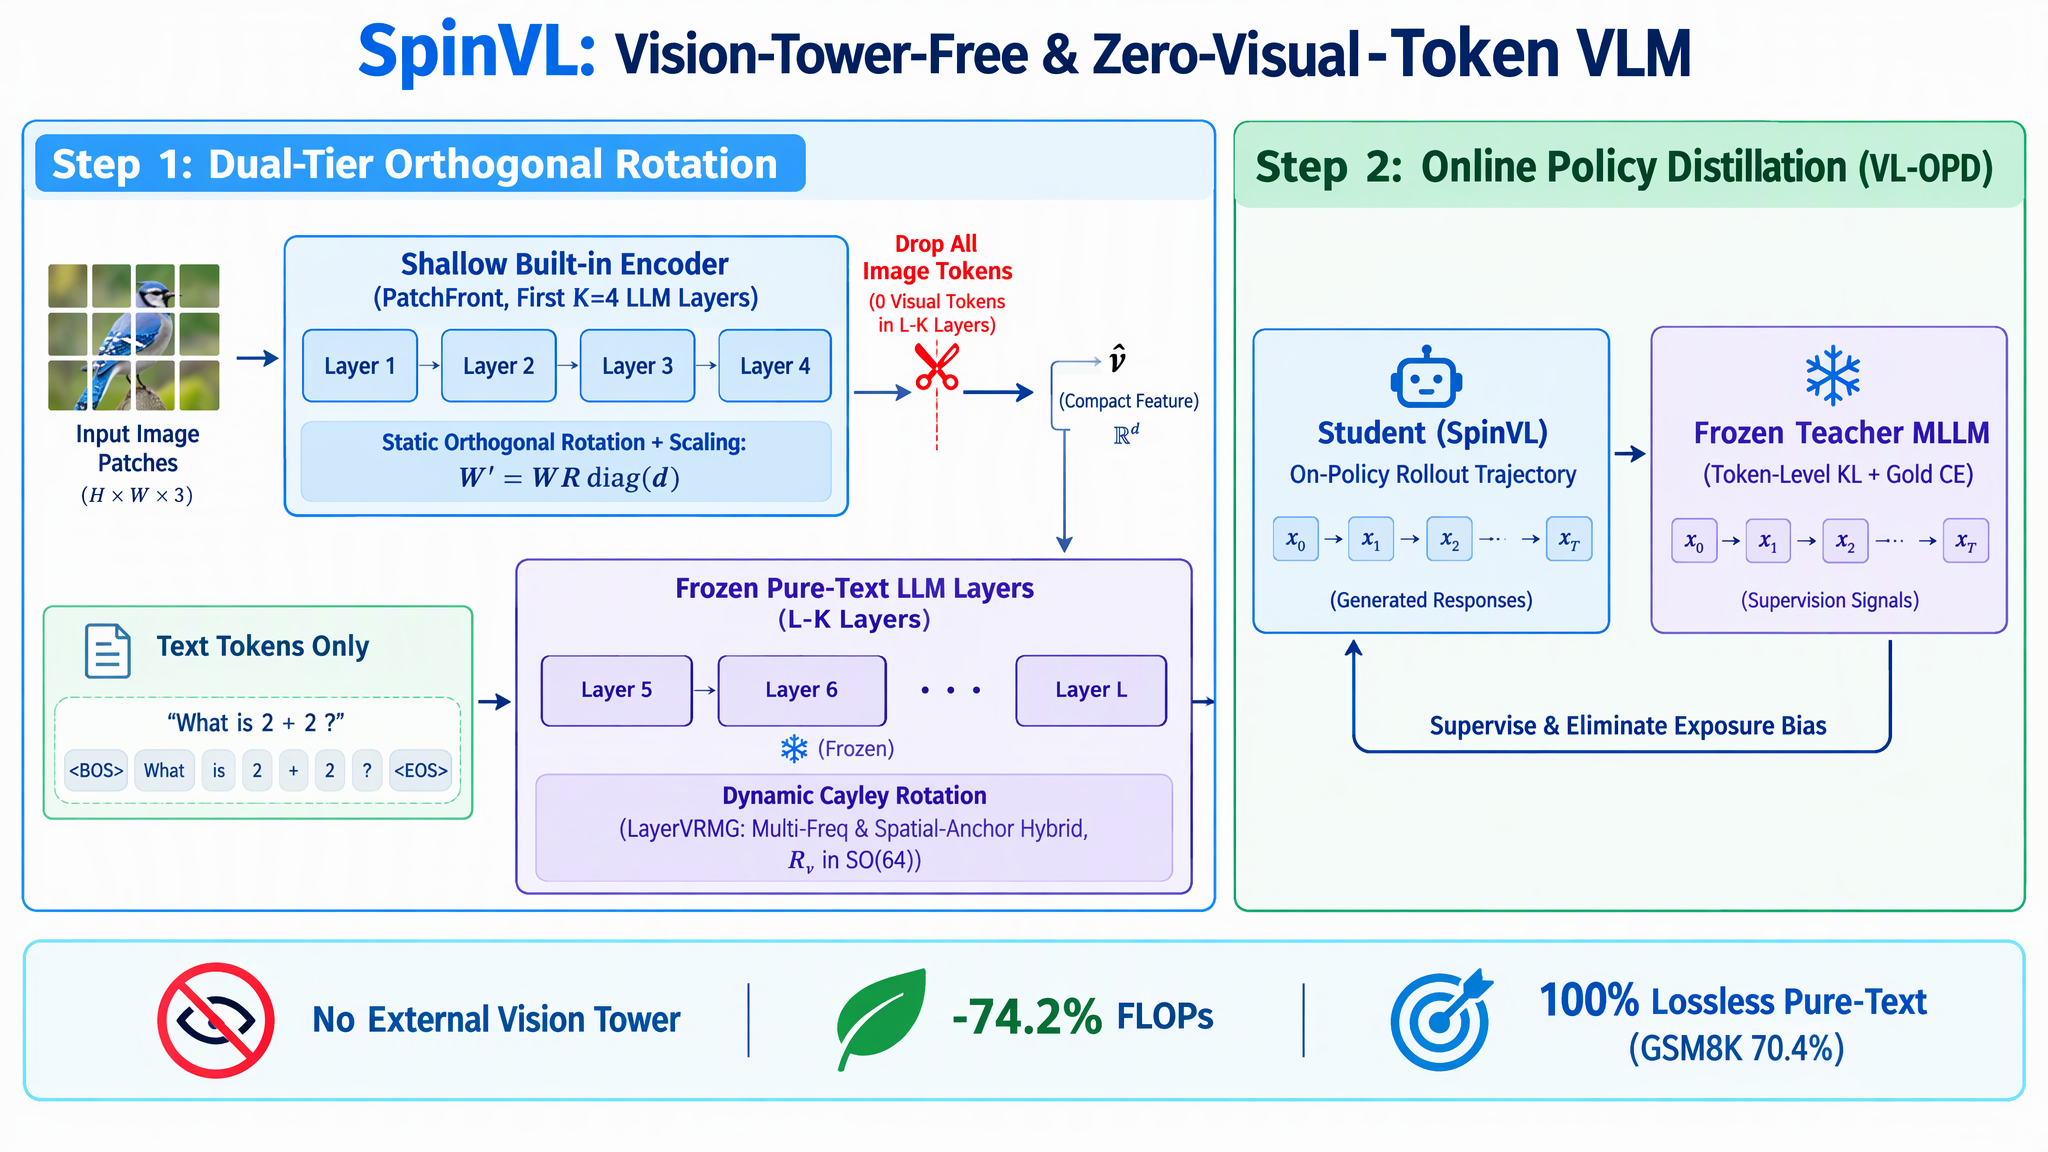
\includegraphics[width=0.98\textwidth]{fig_architecture.png}
\caption{\textbf{Overview of \modelname.} A completely frozen pure-text LLM is
turned into a VLM without any visual token inside the deeper backbone.
\emph{Step~1 (dual-tier orthogonal rotation):} the student's own first
$K{=}4$ layers act as a built-in vision encoder with static Cayley rotation
and channel scaling; all image tokens are discarded after layer $K$, and a
compact cell feature drives dynamic block-diagonal rotations in the remaining
layers. \emph{Step~2 (online policy distillation):} the student samples its
own trajectories and is supervised token-by-token by a stronger VLM, which
removes the exposure bias of teacher-forced training. The text pathway is
never modified, so pure-text behaviour is bit-exact.}
\label{fig:arch}
\end{figure*}

Feeding images to a language model is usually done by concatenation: a vision
encoder, often a full ViT with hundreds of millions of parameters, turns the
image into a sequence of tokens that is prepended to the text and propagated
through every layer of the LLM~\citep{liu2023llava,liu2024improved}. This
recipe is simple and effective, but it couples image resolution to the cost of
the language model. At $4096$ patches, a $1.7$B student with $28$ layers
spends $9.85$ TFLOPs per forward pass, an order of magnitude more than the
text-only model would; the KV cache grows with the same factor. The usual
remedy, fine-tuning the backbone on image-text pairs, trades away a property
that is expensive to recover: the instruction-following and mathematical
ability of the original model.

An appealing alternative is to modulate weights instead of extending the
context. Rotation-based injection~\citep{rose2025} keeps the backbone free of
visual tokens by mapping visual features to block-diagonal orthogonal matrices
that rotate the inputs of linear projections. It inherits the text model
untouched and removes the quadratic cost of long visual sequences. Three
problems remain. First, the method still requires an external vision tower,
which is exactly the component one would like to delete when deploying a
single frozen LLM. Second, images are pooled into one static rotation, so
spatial detail is lost and the model cannot revisit a region. Third, the
model is trained with teacher forcing on ground-truth answers; at inference
time it must consume its own prefixes, and small early errors compound---we
observe degenerate repetitions and missing end-of-sequence tokens.

A parallel line of work replaces the vision tower with the LLM's own early
layers~\citep{vora2025}. This removes the tower but keeps the visual tokens
alive: they travel through all remaining layers, so no compute is saved, and
merging the resulting low-rank adapters into the backbone destroys text
reasoning (GSM8K drops from $70.4\%$ to $0.0\%$ in our controlled experiment).

This paper asks whether one can have all three properties at once: no
external vision tower, no visual token in the deeper backbone, and intact text
ability. \modelname{} answers affirmatively with a two-step framework
(Fig.~\ref{fig:arch}).

\textbf{Step~1: dual-tier orthogonal rotation.} We distinguish two tiers of
adaptation. In the shallow tier, the student's first $K$ layers are
repurposed as a vision encoder using \emph{static} orthogonal rotation
combined with a channel-wise diagonal scaling, which preserves angular
geometry yet, unlike a pure rotation, can rescale singular values. Only
$2.4$M parameters are involved. After layer $K$ every image token is dropped
and a compact set of cell features remains. In the deep tier, those features
generate \emph{dynamic} block-diagonal rotations for the remaining frozen
layers. We propose two complementary generators: a multi-frequency variant
that splits rotation blocks into low-, mid-, and high-frequency bands with
RoPE-style positional encodings, and a hybrid variant that adds a lightweight
cross-attention over a handful of spatial anchors. The two target different
abilities---multi-step diagram reasoning versus fine-grained perception---and
we report both.

Because rotations are applied through a context-local wrapper, the text
pathway is untouched: with the vision branch switched off the model is
bit-identical to the original LLM ($70.4\%$ GSM8K, $71.4\%$ ARC-C). This is
not true for additive adapters or for permanently merged rotations, whose text
accuracy collapses.

\textbf{Step~2: online policy distillation.} Offline teacher forcing trains
the model only on ground-truth prefixes. We therefore let the student roll out
its own answers and ask a stronger VLM to score exactly those tokens with a
full-vocabulary forward KL, anchored by a gold cross-entropy term. Five
hundred steps suffice to raise free-form generation by $+4.1$ to $+9.9$
points across benchmarks and to bring end-of-sequence termination above
$95\%$.

\textbf{Controlled evidence.} All models in our main table share the same
frozen base model, the same training mixture, and the same optimisation
budget; the token-concatenation baseline is retrained by us rather than quoted.
Under this protocol \modelname{} improves the average of perception and
anti-hallucination from $41.35\%$ to $44.37\%$ without any visual token in the
backbone, reaches $35.90\%$ on the average of perception, hallucination and
mathematical reasoning against $35.87\%$ for the token-concatenation
baseline, and, in the tower-free configuration, retains $97.4\%$ of that
baseline's score while using $74.2\%$ fewer FLOPs and running $19.5\%$ faster
at high resolution.

Finally, we characterise the limits of the paradigm instead of hiding them.
By re-training the concatenation baseline on identical data that includes
open-ended chart and document questions, we show that its accuracy on
character-level chart reading and OCR stays flat ($10.32\%$ and $1.10\%$),
while our model stays in the low single digits; adding the same data doubles
our geometry accuracy. Operator-level modulation therefore buys semantic
perception, hallucination resistance and diagram reasoning, but not dense
transcription, which appears to require per-position key-value addressing.

Our contributions are:
\begin{itemize}
\item A dual-tier orthogonal rotation architecture that keeps zero visual
tokens in the backbone and needs no external vision tower, using $2.4$M
static parameters to turn the student's first layers into a vision encoder and
discarding all image tokens thereafter.
\item Multi-frequency and spatial-anchor rotation generators for the deep
tier, together with a modality-decoupled wrapper that makes pure-text
behaviour bit-exact.
\item An online policy distillation stage that repairs autoregressive drift of
rotation-injected models with $500$ steps of on-policy token-level KL.
\item A controlled study against token concatenation, single-frequency
rotation and LoRA-based built-in encoders, covering $0.6$B--$8$B students,
three seeds, compute, latency, text retention, and an explicit statement of
the paradigm's operating envelope.
\end{itemize}
